\documentclass{standalone}
\usepackage{tikz}
\usepackage{ctex,siunitx}
\usepackage{tkz-euclide}
\usepackage{amsmath}
\usetikzlibrary{patterns, calc}
\usetikzlibrary {decorations.pathmorphing, decorations.pathreplacing, decorations.shapes,}
\begin{document}
\small
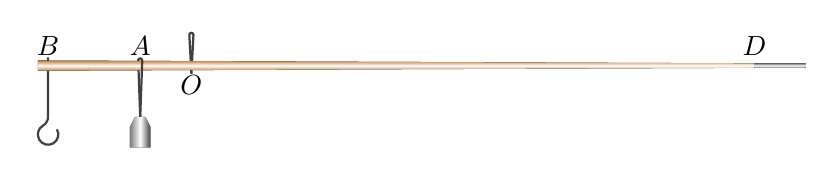
\begin{tikzpicture}[>=stealth,scale=1.3]
  \draw[thick,darkgray](0,-0.08)--(-0.02,0.3)arc(180:0:0.02)--cycle;
  \node at (0,0)[below]{$O$};
  \node at (-1.4,0)[above]{$B$};
  \node at (-0.5,0)[above]{$A$};
  \node at (5.5,0)[above]{$D$};
  \draw [darkgray,thick](-0.52,0.06)--(-0.5,-0.5);
  \draw[thick,darkgray] (-1.4,0.08)--(-1.4,-0.5)arc(0:-60:0.1)arc(120:390:0.1);
  \fill[top color=brown,bottom color=brown,middle color=white]
  (-1.5,0.05)--(6,0.02)--(6,-0.02)--(-1.5,-0.05);
  \fill[left color=gray,right color= darkgray,middle color=white]
  (-0.5,-0.5)--++(-0.05,0)--++(-0.05,-0.1)--++(0,-0.2)--++(0.2,0)--++(0,0.2)--++(-0.05,0.1)--cycle;
  \draw [darkgray,thick](-0.52,0.05)arc(180:0:0.02)--(-0.5,-0.5);
  \fill[top color=gray,bottom color=gray,middle color=white](5.5,-0.02)rectangle(6.0,0.02);
\end{tikzpicture}
\end{document}